\chapter{Fundamentals}
\label{chap:fundamentals}
%background - What do I need to know to understand the thesis?

%%%%%%%%%%%%%%%%%%%%%%%%%%%%%%%%%%%%%%%%%%%%%%%%%%%%%%%%%%%%%%%%%%%%%%%%%
\section{Overview of Organizational Modeling}
\label{sec:overvieworgmodel}
%%%%%%%%%%%%%%%%%%%%%%%%%%%%%%%%%%%%%%%%%%%%%%%%%%%%%%%%%%%%%%%%%%%%%%%%%

%%%%%%%%%%%%%%%%%%%%%%%%%%%%%%%%%%%%%%%%%%%%%%%%%%%%%%%%%%%%%%%%%%%%%%%%%
\section{Related Work}
\label{sec:relatedwork}
%%%%%%%%%%%%%%%%%%%%%%%%%%%%%%%%%%%%%%%%%%%%%%%%%%%%%%%%%%%%%%%%%%%%%%%%%

%%%%%%%%%%%%%%%%%%%%%%%%%%%%%%%%%%%%%%%%%%%%%%%%%%%%%%%%%%%%%%%%%%%%%%%%%
\section{Literature Review}
\label{sec:literaturereview}
%%%%%%%%%%%%%%%%%%%%%%%%%%%%%%%%%%%%%%%%%%%%%%%%%%%%%%%%%%%%%%%%%%%%%%%%%


\section{Organizational Modeling}
\label{sec:orgModeling}

%%%%%%%%%%%%%%%%%%%%%%%%%%%%%%%%%%%%%%%%%%%%%%%%%%%%%%%%%%%%%%%%%%%%%%%%%
\subsection{Organizational Modeling Notation}
%%%%%%%%%%%%%%%%%%%%%%%%%%%%%%%%%%%%%%%%%%%%%%%%%%%%%%%%%%%%%%%%%%%%%%%%%
\hspace{4ex} The Organizational Modeling element notation has been selected as per the guidelines mentioned in the paper by Daniel L.Moody \cite{Moody2009}. Also by observing  the fact that business process modelers are already well-known with the present process modeling notations such as Business Process Modeling Notation 2.0 (BPMN) \cite{bpm2011} and ArchiMate notation\cite{arc2013}, the shape depiction of organizational model elements are designed similar to those existing process notations. 

\hspace{4ex} Due to the importance of shapes in expressing the information visually , the notations are chosen in such a way that each element of Organizational Modeling  differ by shape. Also a legend will be always shown in the modeling notation to denote the meaning of each shape \cite{Moody2009}. As shape plays a primary role in discriminating between different element, organizational model notations are represented through individual shapes like rectangle, double circle, elliptic etc.,. The description of each element in the Organizational Model Notation is shown in the Table \ref{tab:notations}. 

\begin{center}
	\begin{longtable}{p{3cm}p{10cm}p{3cm}}
		\toprule 
		\textbf{Element} & \textbf{Definition} & \textbf{Notation} \\
		\midrule
		\endfirsthead
		Goal 			& Goals are purposeful concrete steps taken to achieve expected outcomes . They reflect the actual intention of an organization.Goals are defined hierarchically, which can contain and extend goals.It is depicted by a double circle. The sub-goals are refined starting from main goal. Goals associated with capabilities are concrete goals and goals that are not associated with capabilities are abstract goals. Abstract goals are represented by dashed double circle and concrete goals are depicted by a solid double circle. & \begin{center} 
\includegraphics[width= 0.07\textwidth]{intentions.png}  \end{center}  \\  
		
		Capabilities	& Organizational capability is the ability to provide business values like software applications, resources, and potential of the actor to make decisions even in changing situations \cite{Stirna2012}. Capabilites are represented by a elliptical circle. Capability is an ability that should be possessed by an Actor or a Resource that work towards achievement of goal.   & \begin{center} 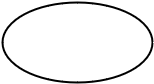
\includegraphics[width= 0.1\textwidth]{capabilities.png} \end{center}   \\
		
		Context				& The environment that forms the setting for an event, statement, or idea, and in terms of which it can be fully understood. There are two Contexts: Initial and Final. The Initial Context is the situation which describes the driving forces that trigger the process to start. The Final Context is the expected situation once the process has finished.Both initial and final context are represented by an hexagonal shape except the final context has thick edges than initial context.  & \begin{center} 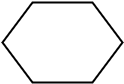
\includegraphics[width= 0.1\textwidth]{context.png} \end{center}  \\
		
		
		Strategy		&  A method or plan chosen to bring about a desired future, such as accomplishment of a goal. Strategies are expressed by rectangles with sharp edges. In the conceptual Organizational Modeling, strategies are self-contained and loosely coupled elements.   & \begin{center} 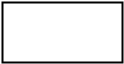
\includegraphics[width= 0.1\textwidth]{strategy.png} \end{center}   \\
		
		Resources					& The people and tools needed to fulfill the middle objectives or those/that work towards the achievement of goal . Resources are represented by a rounded rectangle. Resources are linked to capabilities and actors. & \begin{center} 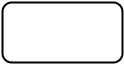
\includegraphics[width= 0.1\textwidth]{resources.png} \end{center}   \\
		
		Actors					& People who participate in the process. Actors are represented by a stick-man and they are linked to resource as actors can be resources. Actors define the strategy and goals.  & \begin{center} 
\includegraphics[width= 0.07\textwidth]{actor.png} \end{center}   \\
		
		Relationship				& A relationship is used specify the fixed links between the elements of the model. Relationship between two elements is represented by a single direction line which represents a sequence.  & \begin{center} 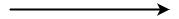
\includegraphics[width= 0.1\textwidth]{relationship.png} \end{center}   \\
		
		
		\bottomrule
		\caption{Informal Process Modeling Notation}
		\label{tab:notations}		
	\end{longtable}	
\end{center}


%%%%%%%%%%%%%%%%%%%%%%%%%%%%%%%%%%%%%%%%%%%%%%%%%%%%%%%%%%%%%%%%%%%%%%%%%
\subsection{Organizational Modeling Notation Example}
%%%%%%%%%%%%%%%%%%%%%%%%%%%%%%%%%%%%%%%%%%%%%%%%%%%%%%%%%%%%%%%%%%%%%%%%%
\hspace{4ex} The concept of Organizational Model Notations can be explained with the following manufacturing scenario. ABC Ltd. is a budding computer technology company which designs, develops, manufactures and sells personal computers, tablets and laptops. The CEO's goal of the quarter is to increase the revenue and number of unit sales. The initial context describes the situation that motivates to start the process. The final context describes the situation that is achieved once the process completed successfully. Goals connect initial context definitions with final context definitions \cite{Sungur2014a}. The sub-goals are the intermediate goals which describes the expected outcome in a measurable form. Goals are reached through strategy implementation which is plan of action designed to meet a goal. 

\hspace{4ex} The example scenario ABC Ltd. helps in understanding the organizational modeling i.e., how organization's higher level goal can be achieved by amalgamation of specific, measurable and realistic sub-goals. . The whole view has been divided into Goal view and Strategy view. The \textit{Goal View} shown in the Figure\ref{fig:goalview} provides only the details of goal and its associated strategies. There can be multiple strategies followed to achieve a goal. The \textit{Strategy View} shown in the Figure\ref{fig:strategyview} connects big picture of each strategy with individual goals that has to be carried out. In Organizational Process Modeling, strategies are self-contained and loosely coupled. So that when we extract only the strategies from Organization Process Modeling it would be similar to Informal Process Essential Modeling. 

\hspace{4ex} The Strategy view  in the Figure\ref{fig:strategyview} depicts big picture of each strategy. Strategies are associated with both goals and capabilities. Capabilities are related to goals and resources. As each goal needs certain capability to successfully execute the goal they both are connected using the verb \textit{"requires"}. Resources are the potential holder of the capability i.e., to satisfy a capability we need resources. The capability and its associated resources are linked using the verb \textit{"satisfied-by"}. 


\begin{figure}
	\centering
	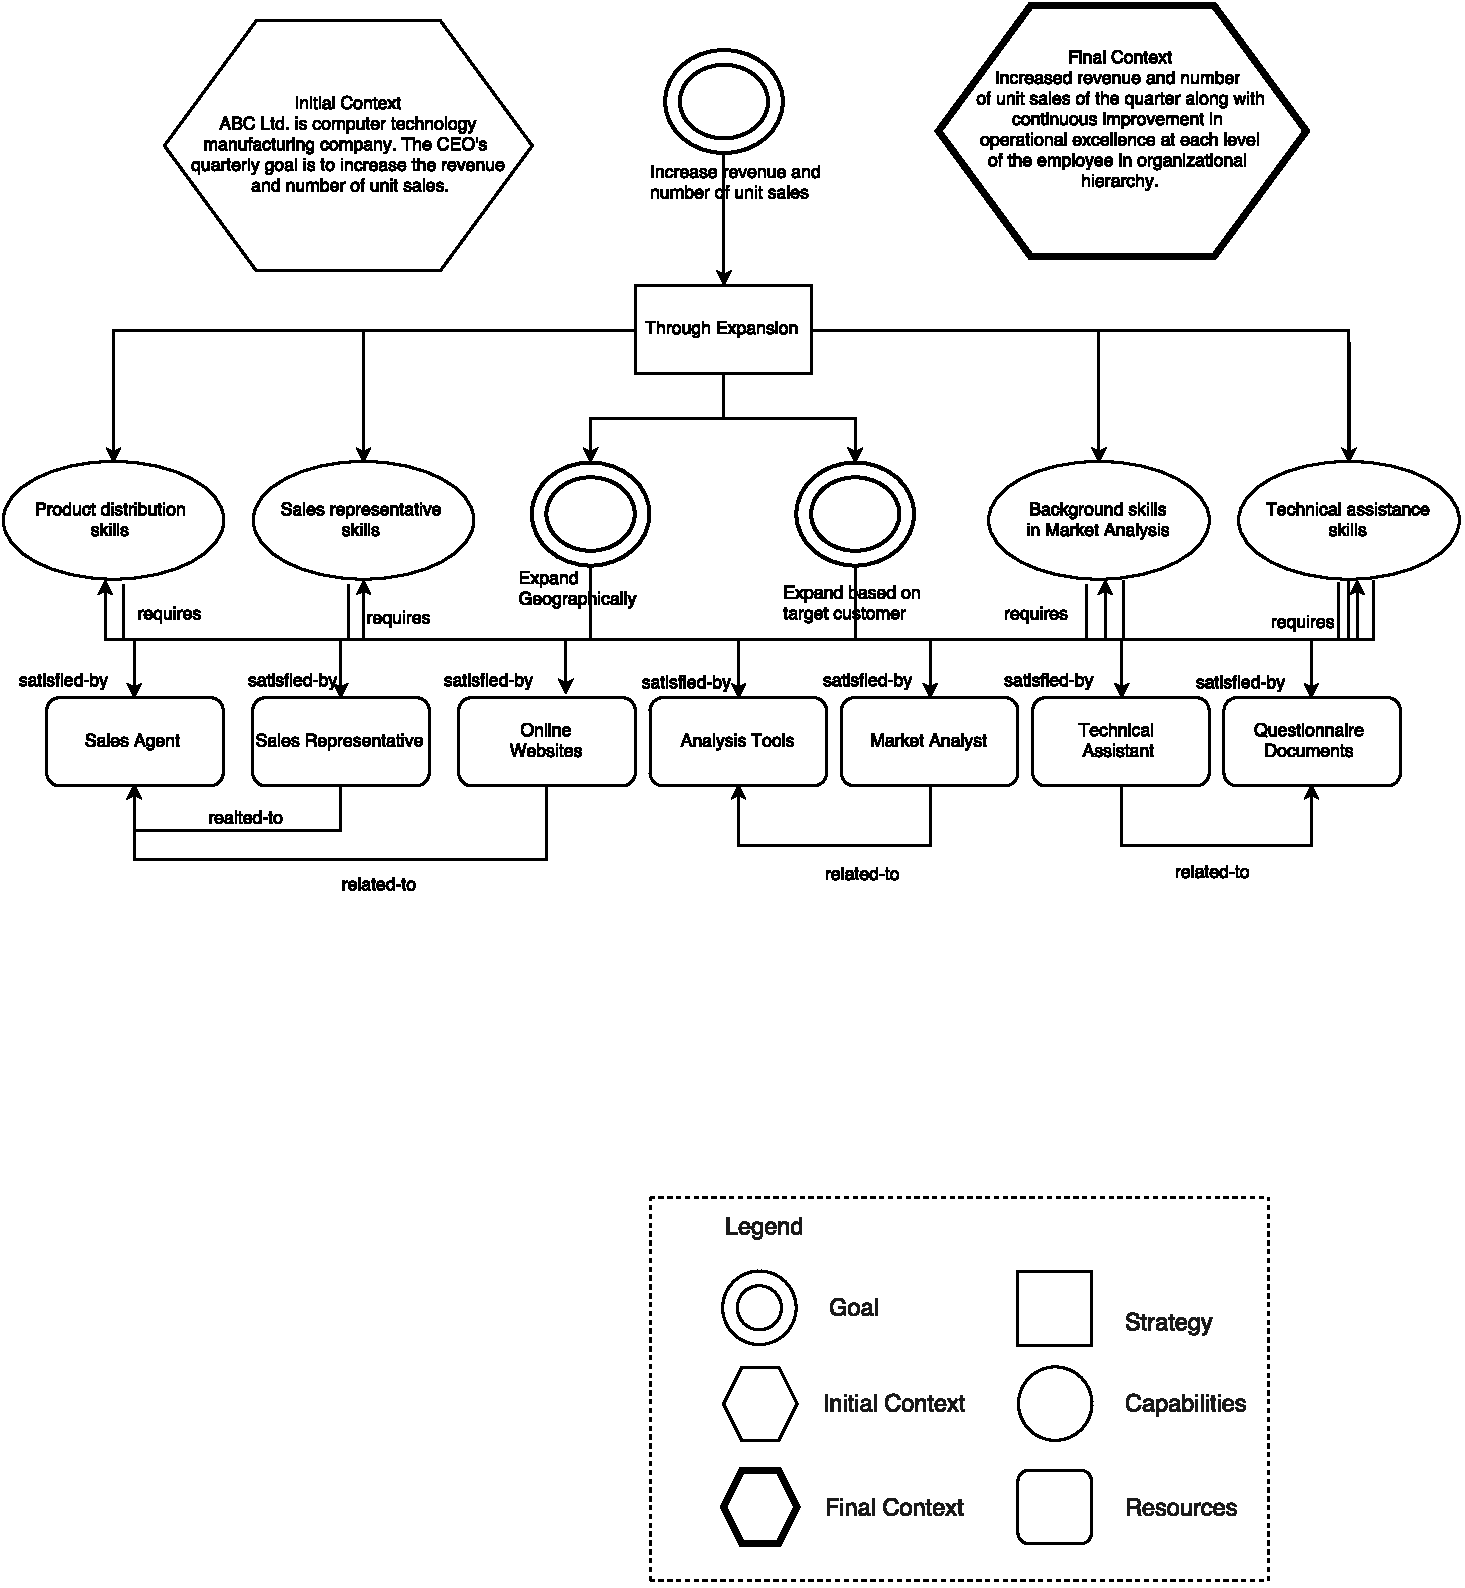
\includegraphics[width=\textwidth]{StrategyView.pdf}
	\caption{Strategy View}
	\label{fig:strategyview}
\end{figure}

\begin{figure}
	\centering
	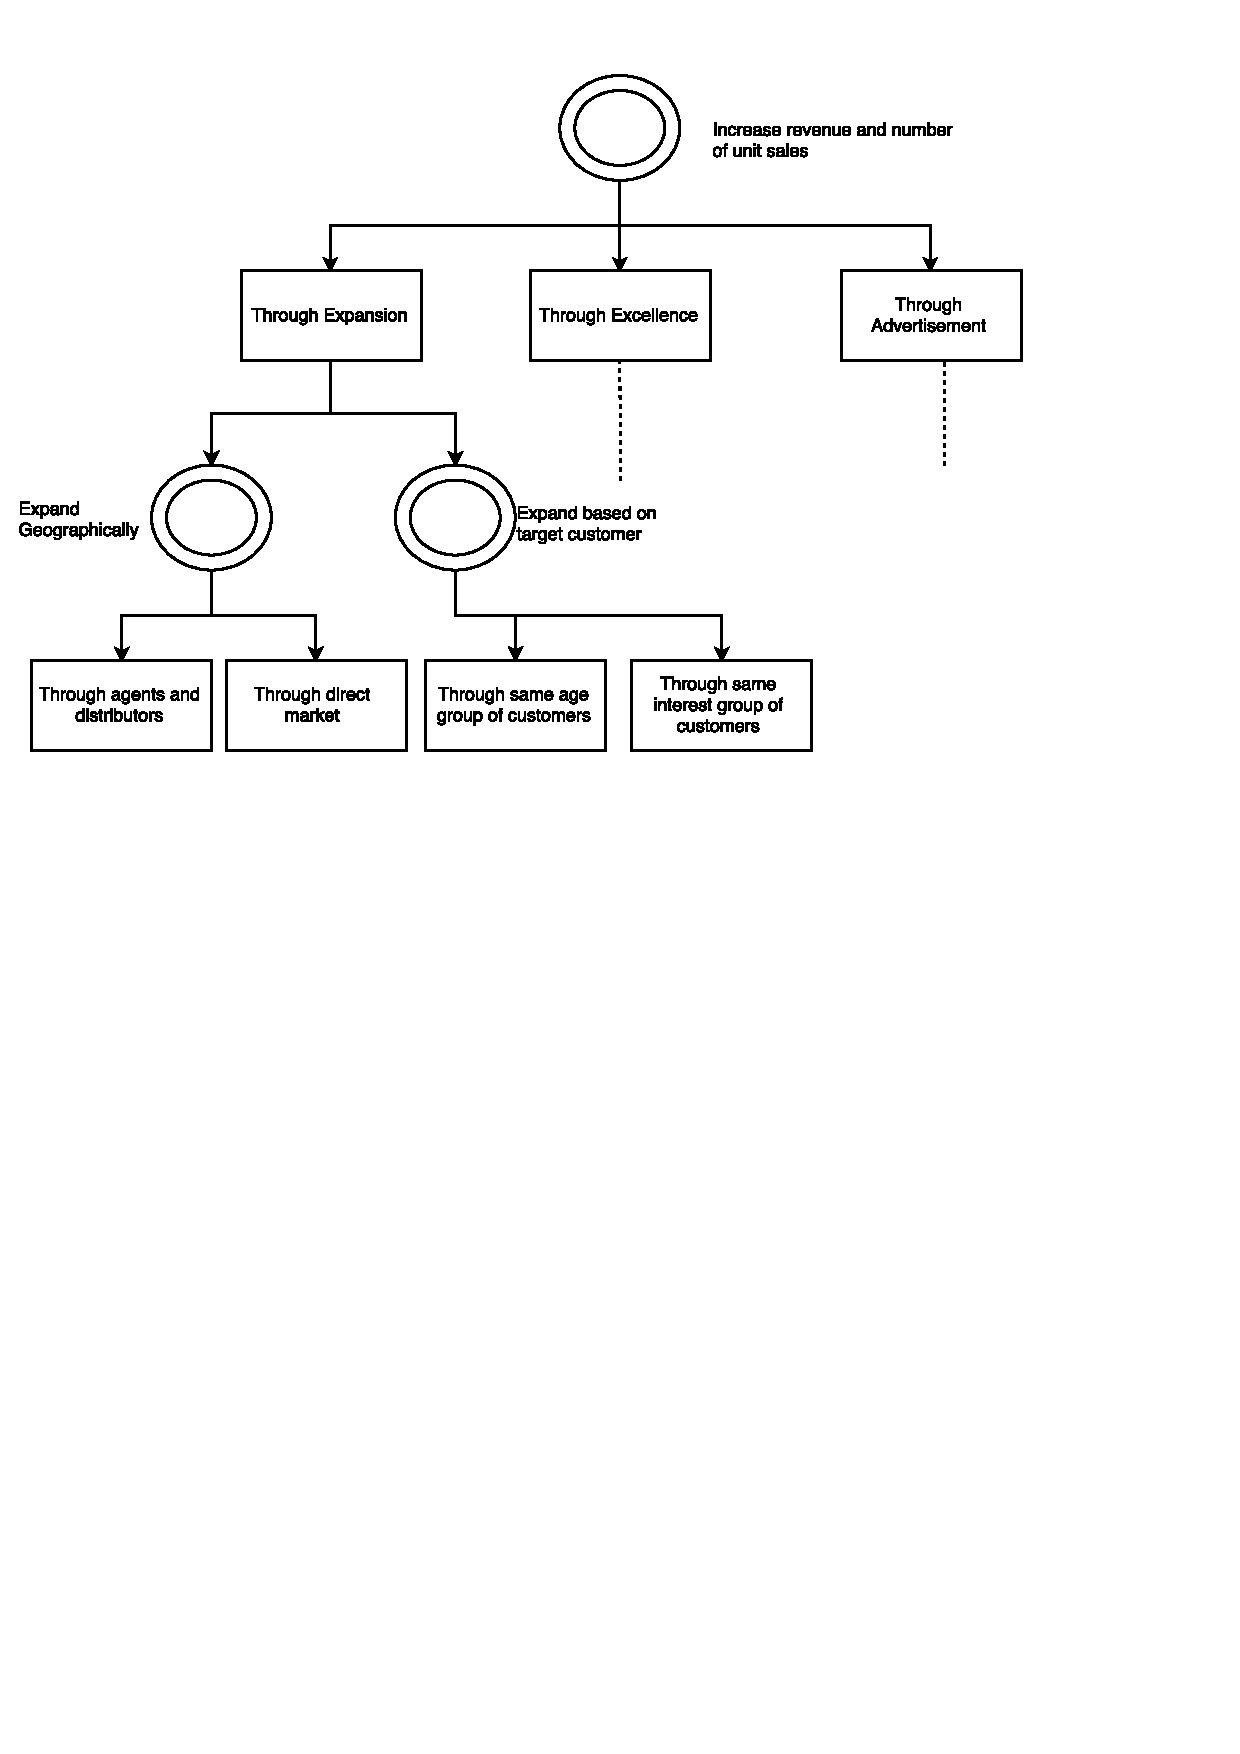
\includegraphics[width=\textwidth]{GoalView.pdf}
	\caption{Goal View}
	\label{fig:goalview}
\end{figure}

%%%%%%%%%%%%%%%%%%%%%%%%%%%%%%%%%%%%%%%%%%%%%%%%%%%%%%%%%%%%%%%%%%%%%%%%%
\subsection{Organizational Modeling Process Representation}
%%%%%%%%%%%%%%%%%%%%%%%%%%%%%%%%%%%%%%%%%%%%%%%%%%%%%%%%%%%%%%%%%%%%%%%%%
\begin{figure}
	\centering
	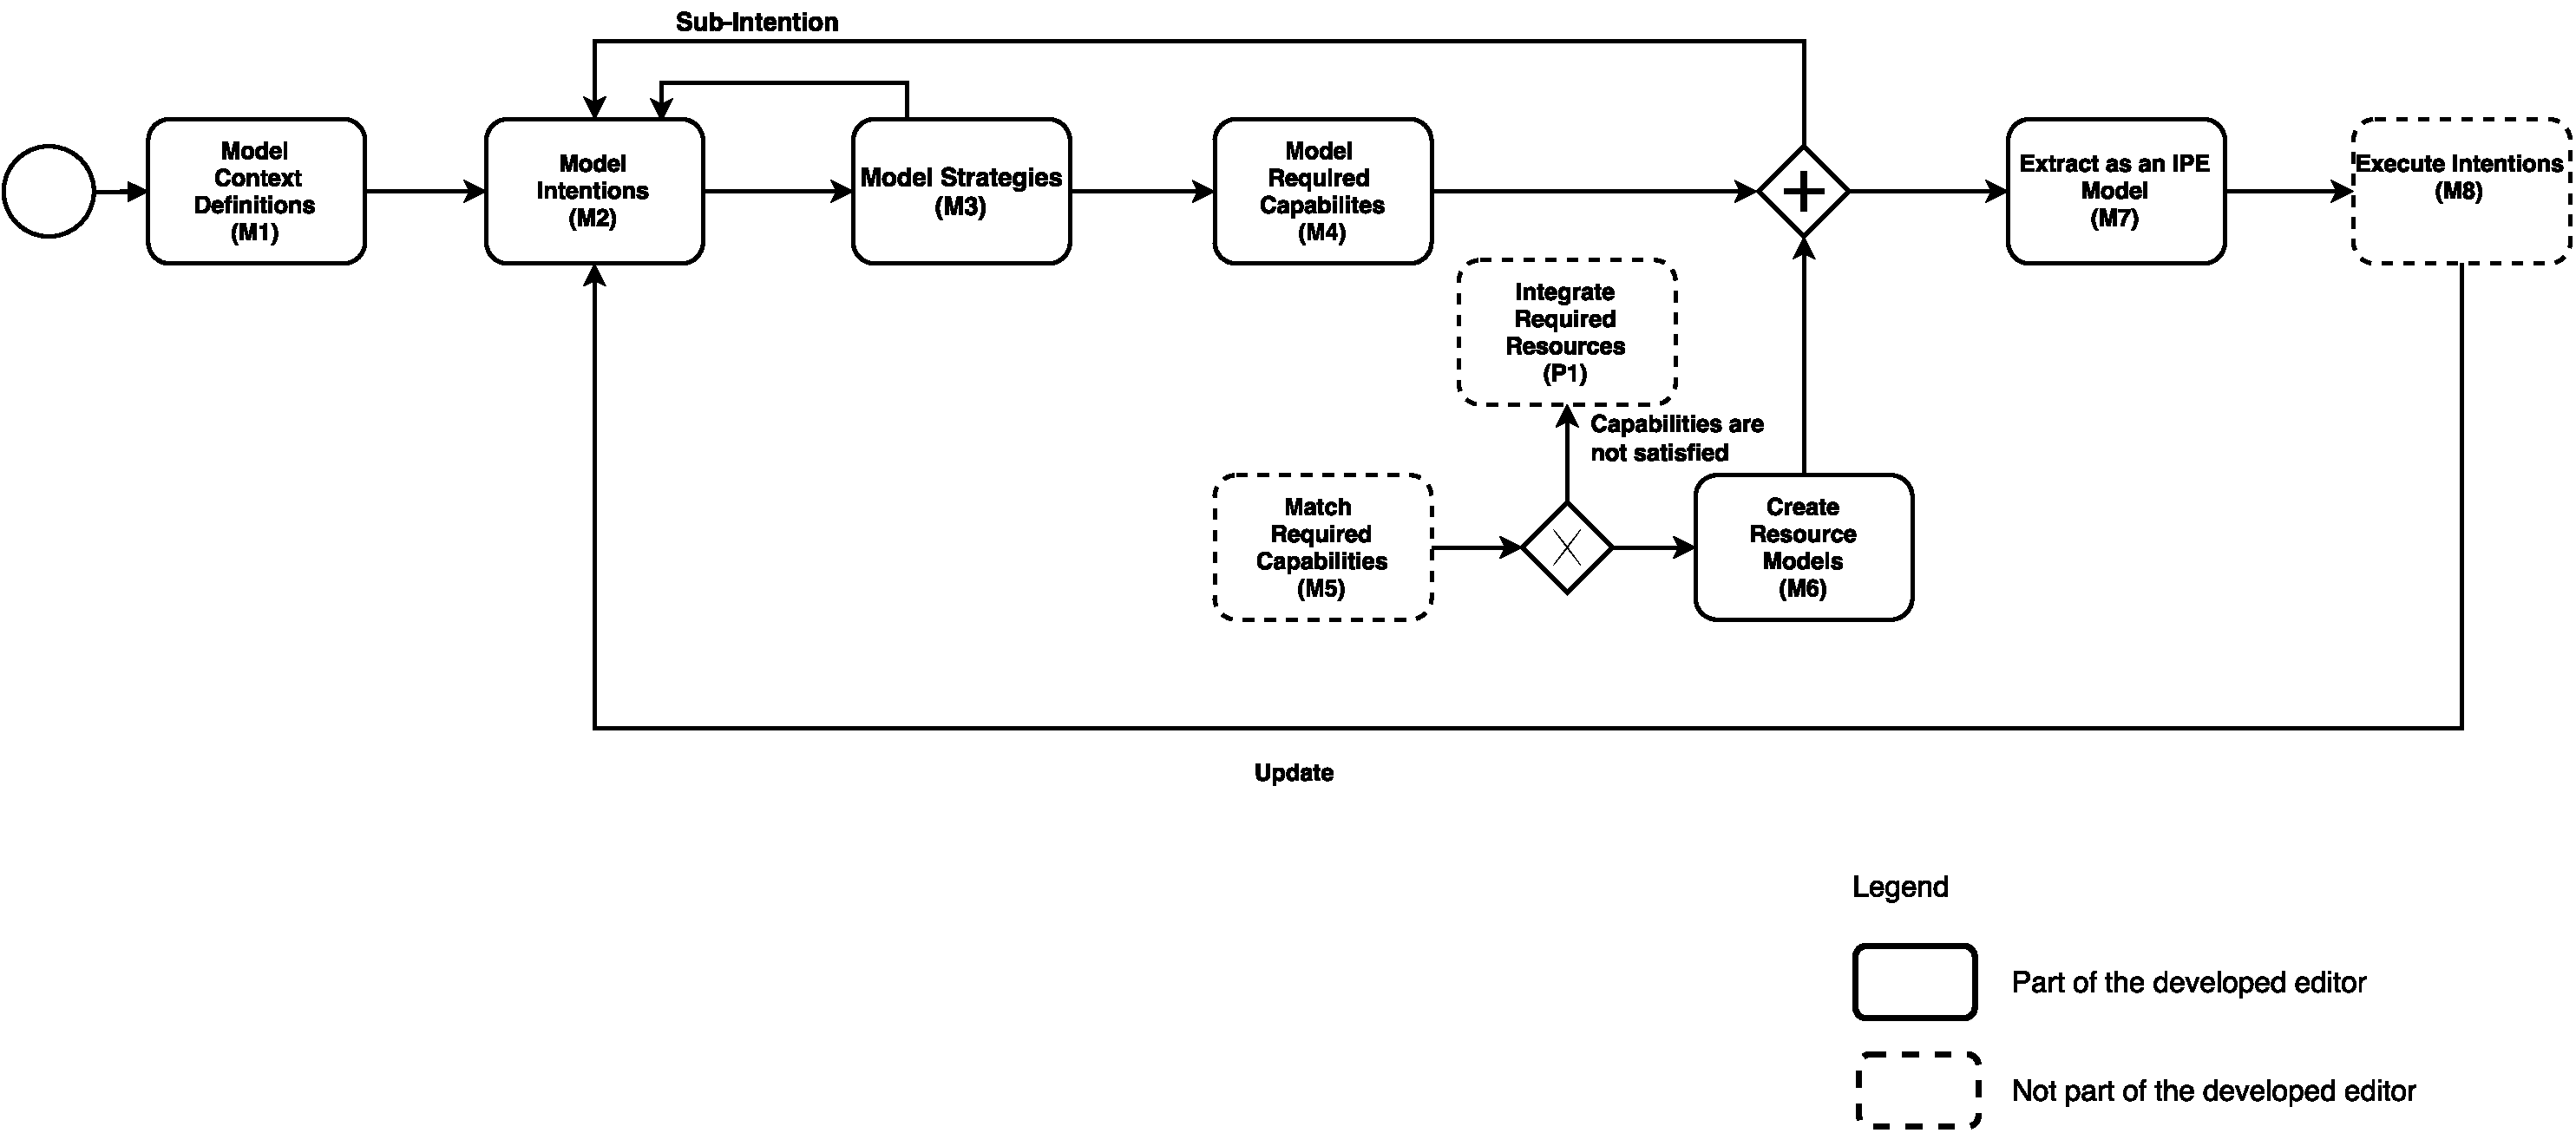
\includegraphics[width=\textwidth]{processmodeling.pdf}
	\caption{Process Modeling Diagram}
	\label{fig:processdiagram}
\end{figure}

\hspace{4ex} Organizational Process Modeling depicted inFigure \ref{fig:processdiagram} captures required organizational capabilities that are satisfied by resource models  to enable the achievement of organizational goals in certain context definitions through a strategy. It is a top-down approach, i.e., first goals are defined and then sub-goals  are defined by refining main goal. Goals connect initial context definitions with final context definitions through a strategy.  To understand the definition of Organizational Process Modeling we need to interpret the Organizational Process Modeling Representation shown in Figure\ref{fig:processdiagram}. 

\hspace{4ex} The Organizational Process Modeling start with modeling of organizational goal (M1). Once the goal has been modeled, the second step is to model the strategies which can be a multi-instance strategy model(M2). The next step is to model the context definitions (M3.1), required organizational capabilities (M3.2) and refining the sub-goals from main goal in parallel. Once the required capabilities(M4) are matched by required resources(P1), modeling of resources(M5) can be done.  Based on created resource models (M5) and modeled context definitions(M3.1), strategies can be executed. The organizational goals would be iteratively updated supported to strategy execution.  


%%%%%%%%%%%%%%%%%%%%%%%%%%%%%%%%%%%%%%%%%%%%%%%%%%%%%%%%%%%%%%%%%%%%%%%%%
\subsection{Organizational Modeling Entity Representation}
%%%%%%%%%%%%%%%%%%%%%%%%%%%%%%%%%%%%%%%%%%%%%%%%%%%%%%%%%%%%%%%%%%%%%%%%%

\begin{figure}
	\centering
	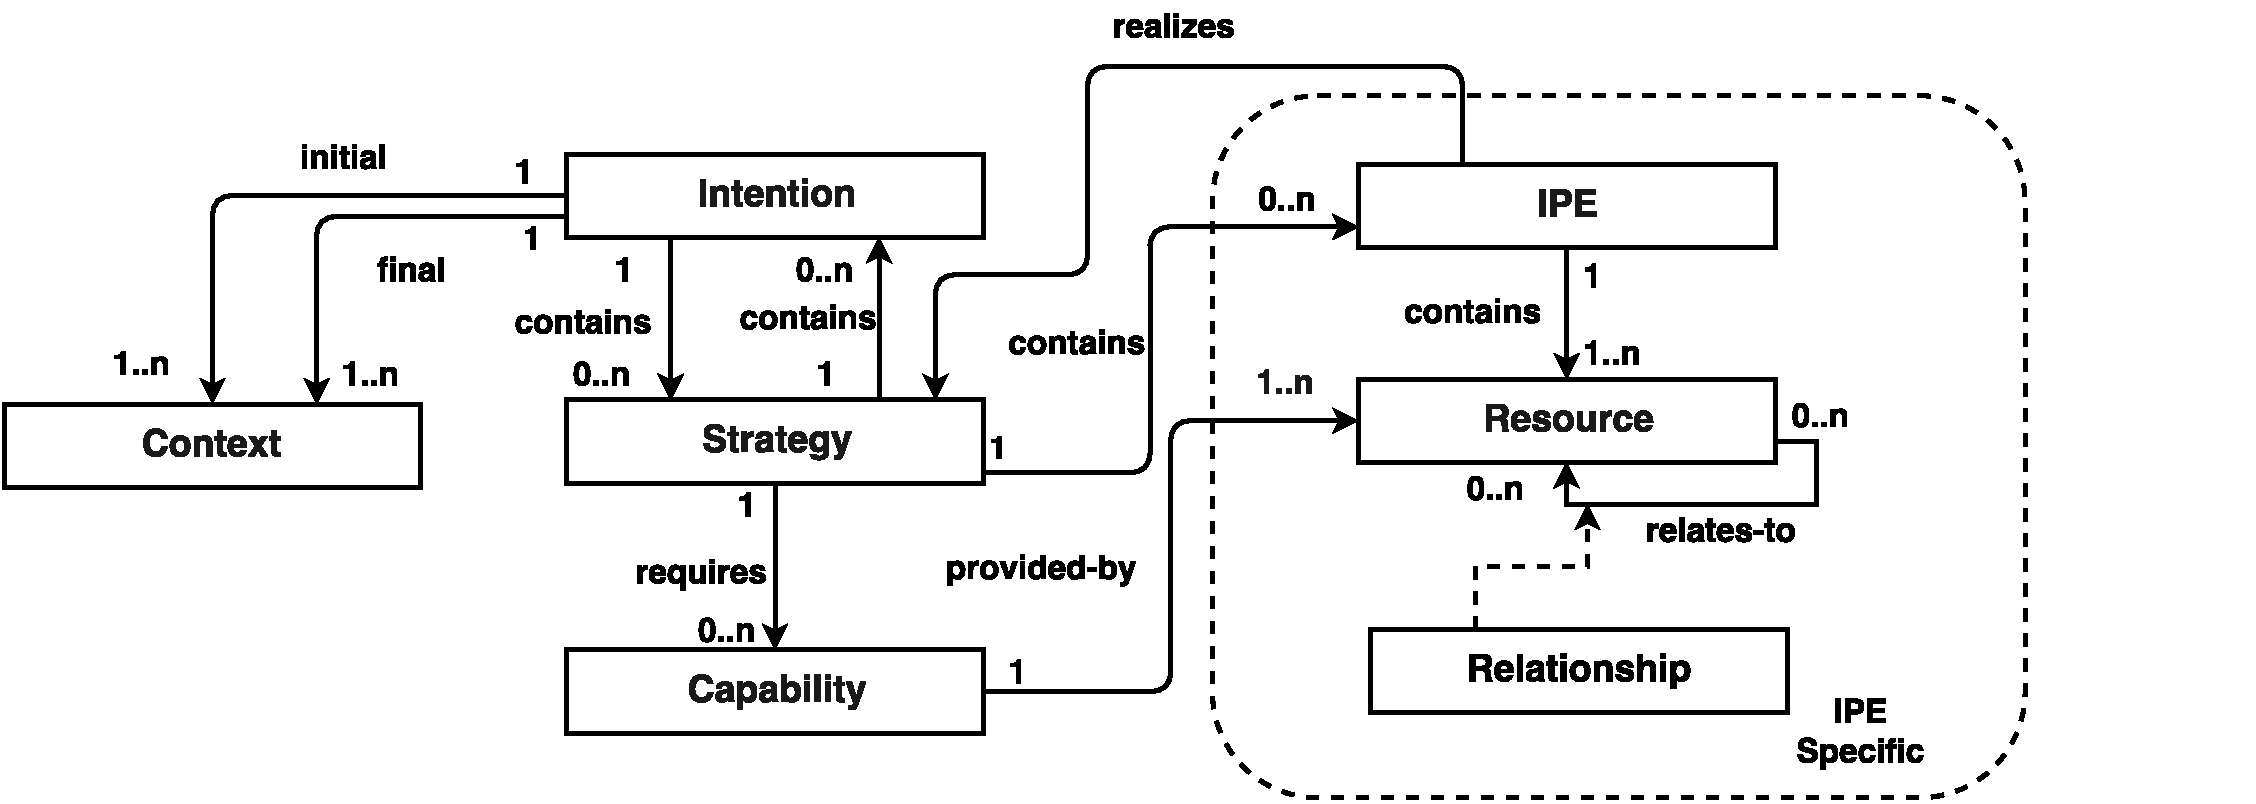
\includegraphics[width=\textwidth]{entity.pdf}
	\caption{Organizational Modelling Meta-Model}
	\label{fig:metamodel}
\end{figure}

\hspace{4ex} The conceptual entity model of goals is shown in the \ref{fig:metamodel}. This model shows that top level goal is refined into sub-goals. A goal can be achieved through a strategy which is a plan of action designed to meet a goal. It also describes a set of interrelated resources which work together to achieve a collective goal. As reported by Sungur et al. \cite{Sungur2014a}, the concept of IPE provides an agent-based approach i.e., human performers are considered as agents who execute the processes autonomously. Based on the approach \cite{Sungur2014a} we provide a goal-oriented approach based on goals.

\hspace{4ex} Organizational Process Modeling  has \textit{Resources} which are used to achieve the goals. Organizational Process Modeling is Resource-centric approach as they support processes by providing required resources and thrives to successfully execute the processes by using qualified autonomous agents, i.e., actors under certain \textit{context definitions}.  Resources can be anything like people, IT tools, data that are used to accomplish the objectives.Emerging goals can result in the requirement of new capabilities, i.e., resources. A more specific type of resource is the type \textit{Actor}, which typically refers to human performers who autonomously and collaboratively conclude an organizational process using other available Organizational Process Modeling Resources.Actors work towards the goals defined in the process. Resource models are optional to make precise definitions of resources needed.

\hspace{4ex} In Sungur et al \cite{Sungur2014a} work, the concept of \textit{Informal Process Support Model} IPSM has been introduced which is to make use of existing knowledge of human performers. Here the initial creator of the model is experienced human performers. Based on their experience, they add relevant  resources of an informal process. Each of the resources has inter relationships among the resources themselves. The models are generated at runtime based on the interactions and activities of corresponding human performers. 

\hspace{4ex} An informal process targets for accomplishment of a goal. The goals can be refined by defining sub-goals, which can be defined recursively as independent informal processes. The goal-based approach enables describing processes declaratively, i.e., without describing \textit{how} the intention is achieved, and providing only information about \textit{what} is achieved. Thus, to avoid predefined business logic in the representations of informal processes. 

\hspace{4ex} Each informal process starts from an initial context, i.e., \textit{IPE Context} and aims to achieve a goal. After accomplishing the goal, there is a resulting context called as final context. Each Resource can be related to another Resource in the context of an informal process using predefined or custom \textit{Relationships}.

%%%%%%%%%%%%%%%%%%%%%%%%%%%%%%%%%%%%%%%%%%%%%%%%%%%%%%%%%%%%%%%%%%%%%%%%%
\subsection{Requirements Supporting Organizational Modeling}
%%%%%%%%%%%%%%%%%%%%%%%%%%%%%%%%%%%%%%%%%%%%%%%%%%%%%%%%%%%%%%%%%%%%%%%%%

\hspace{4ex} \textbf{Requirement 1 (R1)}: \textit{Organizational goal transparency.} A goal can be broken down into definitive actionable components, or sub-goals, upon which individual resources can act. When these lower level sub-goals are made  achievable for individual resources, they can be combined to provide successful execution of higher level goal. Different organizational members can observe lower level and higher level goals in their organizations. Goals are traceable in the different levels of the organizational hierarchy. This kind of transparency within an organization reduces inefficiencies in goal execution, and is a key factor in attracting and retaining high  performers in the labor market \cite{McManus2007}.Requirement R1 has to be satisfied in the modeling time of the process itself as the framing of goals, sub-goals, strategies are done during the modeling time .

\hspace{4ex} \textbf{Requirement 2 (R2)}: \textit{Organizational goal resource-based cost estimation.}Linking goals with capabilities and with resources enable us a cost estimation for each goal. Cost is estimated in a recursive manner. Cost of a goal is calculated as follows  
\begin{equation}
	Gc = \sum SGc_i + \sum_{for\hspace{0.1cm}every\hspace{0.1cm}capability} (min Sr + max Sr)/2
\end{equation}
To incorporate the cost estimation of goals, we have to understand the recursive structure of the goals associated with capabilities.Since goals are defined hierarchically, they can contain and extend goals. Here strategy represents a means for achieving the goal. Further on, the cost of a strategy can be analyzed using the costs of derived  goals, and so on. Including resources cost in goal cost calculation is important. The recursion is stopped when the goal derivation process reaches the operational
level. At the moment a  goal is achieved, some resources should be allocated to maintain the desired state (goal maintenance costs)\cite{Mandic2010}. Allocation of resources is mainly done at the operational level, Requirement R2 has to be satisfied in the run time of the process.

\hspace{4ex} \textbf{Requirement 3 (R3)}: \textit{Organizational goal achievability estimation.}The sub-goals are projections of their super goals, and satisfaction of the sub-goals ensures satisfaction of the super goals. Hence validity of an organizational goal is achievable when the goals can be refined by defining sub-goals, which can then be defined recursively as independent informal processes. Lower-level requirements can be validated against higher-level goals, thus enabling validation of strategic alignment of  higher level goals. The objectives of business strategy are found in the highest levels of the goal model.\cite{Bleistein2006}.Requirement R3 has to be satisfied during the modeling time of the process as goal achieveability estimations are done before starting the execution of the goal.

\hspace{4ex} \textbf{Requirement 4 (R4)}: \textit{Goal-oriented working style.}As each member of the organization is aware of the higher level and lower level goals and he can engage for these explicit goals. Goal orientation is the degree to which a person or organization focuses on tasks and the end results of those tasks. Strong goal orientation advocates a focus on the ends that the tasks are made for instead of the tasks themselves and how those ends will affect either the person or the entire company. Those with strong goal orientation will be able to accurately judge the effects of reaching the goal as well as the ability to fulfill that particular goal with current resources and skills \cite{Lacom}. The distinction between explicit knowledge of each sub goals should not be seen as a division but rather as a continuum which aligns towards achieving the higher level goal . Thought Requirement R4 itself has sub-requirement of R1, R4 has to be done at the run time which makes it distinct from the Requirement 1.

\hspace{4ex} \textbf{Requirement 5 (R5)}: \textit{Social organizational modeling.}Different members of an organization participate to create organizational goals, as a result goals are shaped based on all members but directed by the executives. The  social  extension  of  a  business  process  can  be  regarded  as  a  process optimization phase, where the organization seeks efficiency  by  extending  the  reach  of  a  business  process  to  a  broader  class  of  stakeholders\cite{Brambilla2012}.Requirement R5 would be done at the run time as the input from different members of the organization provided during the process execution.


\begin{table} [htbp]
	\centering
	\begin{tabular} {p{4cm}p{3cm}p{9cm}}
		\toprule
		\textbf{Requirements}                                                      & \textbf{Requirement Satisfaction Time} & \textbf{Sub - Requirements}    \\
		\midrule                                                                                                               
		Requirement 1 (R1)                    & Modeling time                 &\begin{tabular}[c]{@{}l@{}}1. Main goal can be refinable into sub-goals.\\ 2. Organizational members can view the goals \\ at different levels.\end{tabular}                \\ 
		
		Requirement 2 (R2)                      & Run time               &\begin{tabular}[c]{@{}l@{}}1. Goal cost estimation that includes all recursive \\ sub-goals and resources.\\ 2. Cost estimation including the strategy. \end{tabular}                \\         
		
		
		Requirement 3 (R3)                     & Modeling time            &\begin{tabular}[c]{@{}l@{}}1. Each sub-goal should be achievable and valid.     \end{tabular}                \\      
		
		Requirement 4 (R4)                     & Run time               &\begin{tabular}[c]{@{}l@{}}1. Satisfaction of R1.\\  2.  Understanding of the goals and \\ how they can be reached.   \end{tabular}                \\                         
		
		
		
		Requirement 5 (R5)                      & Run time                 &\begin{tabular}[c]{@{}l@{}}1. Satisfaction of R1.\\  2. The output of goal is based on the inputs \\ provided by different members of the organization.   \end{tabular}                \\     
		
		\bottomrule
	\end{tabular}
	\caption{Sub Requirements}
	\label{tab:subrequirements}
\end{table}